%% LaTeX2e class for student theses
%% sections/apendix.tex
%% 
%% Karlsruhe Institute of Technology
%% Institute for Program Structures and Data Organization
%% Chair for Software Design and Quality (SDQ)
%%
%% Dr.-Ing. Erik Burger
%% burger@kit.edu
%%
%% Version 1.3.3, 2018-04-17

\iflanguage{english}
{\chapter{Appendix}}    % english style
{\chapter{Anhang}}      % german style
\label{chap:appendix}

\section{Semi-structured interview questionnaire}
\label{sec:semi_structured_interview_questionnaire}

\paragraph{Begrüßung - 3 Min}

\begin{itemize}
\item Sick für die Zeit bedanken
\item Vorstellung meiner Arbeit: 
Ich untersuche, wie man die Patent-Landscaping-Aufgabe unterstützen kann. 
Ich werde eine Lösung zu der Datenverarbeitung, die hinter den Kulissen passiert, anbieten, aber vor allem zu der Visualisierung. 
Mein Fokus liegt auf der Interaktion - wie genau man das Wichtigste aus den Daten rausholen kann.
\item Ziels des Gesprächs erklären: Ich möchte verstehen, wie man mit den Daten interagiert. 
Nicht der Benutzer wird getestet, sondern das System. 
Es gibt keine richtigen und falschen Antworten.
\item Ich möchte gerne unser Gespräch aufnehmen -  mit einem Mikrofon, aber ohne eine Kamera. 
Das ist dazu da, dass wir frei reden können und ich nicht die ganze Zeit nur am Notizenmachen bin. 
Die Aufnahme kann nach Wunsch jederzeit gestoppt werden, genauso wie das ganze Interview. 
Dadurch entstehen dem Teilnehmer keine Nachteile. 
\item Darlegen, wie die Daten benutzt werden: Ich werde anhand von der Aufnahme unser Gespräch transkribieren und danach die Aufnahme löschen. 
Selbstverständlich werden die Daten nicht an Dritte weitergegeben. 
Ich werde sie nur im Kontext der Masterarbeit benutzen und möchte gerne das, was Sie sagen, in meiner Arbeit zitieren.
\item Haben Sie Fragen zur Organisation?
\item Einverständniserklärung unterschreiben lassen
\item Aufnahme starten
\end{itemize}

\paragraph{Aufwärmfragen - 5 Min}

\begin{itemize}
\item Stellen Sie sich bitte vor.
\item Was ist Ihr beruflicher Hintergrund (in welchen Branchen haben Sie gearbeitet, wie lange)?
\item Wie sieht Ihr typischer Arbeitsalltag aus?
\item Wie ist Ihr Verhältnis zur Technologie allgemein? Wie vertraut sind Sie mit Technologie?
\item Wie lange beschäftigen Sie sich schon mit Patentenanalyse?
\end{itemize}

\paragraph{Hauptteil - 45 Min}

\begin{itemize}
\item Welche Programme benutzen Sie normalerweise in der Arbeit? (zusätzlich zu STN AnaVist)
\item Wie ist die Aufteilung zwischen allen Tools (Zeit, Aufwand)?
\item Können Sie mir bitte von ihrem letzten erstellten Landscape erzählen?
\begin{itemize}
\item In welcher Form kommt die Aufgabenstellung für ein Landscape?
\item Welche Bedürfnisse haben die Kunden, die Landscapes beantragen?
\item Wie lange dauert es, einen Patent Landscape Bericht zu erstellen?
\item Wie viele Berichte haben Sie ca. schon erstellt?
\item Wie umfangreich ist das Ergebnis?
\item Welche Grafiken (Typ, Achsen) kommen normalerweise in einem Bericht vor?
\item Wie finden Sie die passenden Suchanfragen?
\begin{itemize}
\item Wie lang und komplex sind die Anfragen?
\item Wie viele Treffer ergibt die Suche?
\item Relevanz der Ergebnisse?
\end{itemize}
\item Wie aussagekräftig sind die Beschriftungen der Cluster im Themescape?
\item Gibt es mehrere Abstraktionsebenen bei der Suche? Wenn ja, wie unterscheiden sie sich? (Sublandscapes)
\item Worauf achten Sie bei der Aufgabe?
\begin{itemize}
\item Was für eine Bedeutung haben die Verbindungen zwischen einzelnen Patenten (Zitierung, Patentfamilie, gemeinsamer Autor oder Assignee)?
\item Was für eine Bedeutung hat die zeitliche Entwicklung?
\item Was für eine Bedeutung hat die hierarchische Klassifikation?
\item Welchen Einfluss hat Concept Frequency?
\end{itemize}
\end{itemize}
\item Gibt es etwas, was Sie persönlich am existierendem System stört?
\item Wie unterscheidet sich die Patentsuche für verschiedene Themengebiete? Gab es Fälle, wo es besonders gut oder besonders schlecht funktioniert hat?
\item Gibt es etwas, was Sie gelernt haben nach einigen erstellten Landscapes?
\item Gibt es interessante Geschichten/Anekdoten, die sie teilen wollen?
\item Haben Sie sich mit Menschen ausgetauscht, die andere Tools verwenden? Wie waren ihre Erfahrungen?
\end{itemize}

\paragraph{Ausblick für die Zukunft - 3 Min}

\begin{itemize}
\item Was wäre ein perfektes System für Patent Landscaping?
\item Abschluss - 3 Min
\item Gibt es sonst etwas, was Sie mir mitteilen wollen?
\item Haben Sie Fragen an mich?
\item Bedanken und verabschieden
\item Aufnahme stoppen
\item Hauptgedanken notieren
\end{itemize}

\section{SQL query for the 3D printer dataset}
\label{sec:3d_printer_query}

\begin{verbatim}
SELECT DISTINCT p.publication_number            
FROM
    `patents-public-data.patents.publications` p
    LEFT JOIN UNNEST(p.cpc) AS cpc_code,
    UNNEST(p.title_localized) AS title,
    UNNEST(p.abstract_localized) AS abstract,
    UNNEST(p.ipc) AS ipc_code              
WHERE
    title.language = 'en' AND abstract.language = 'en'
    AND 
    (
         REGEXP_CONTAINS(abstract.text, r'3D') OR REGEXP_CONTAINS(title.text, r'3D')
      OR REGEXP_CONTAINS(abstract.text, r'3-D')  OR REGEXP_CONTAINS(title.text, r'3D')
      OR REGEXP_CONTAINS(abstract.text, r'3-dimension') 
      OR REGEXP_CONTAINS(title.text, r'3-dimension')
      OR REGEXP_CONTAINS(abstract.text, r'3 dimension') 
      OR REGEXP_CONTAINS(title.text, r'3 dimension')
      OR REGEXP_CONTAINS(abstract.text, r'three dimension') 
      OR REGEXP_CONTAINS(title.text, r'three dimension')                
    )
    AND 
    (
        REGEXP_CONTAINS(abstract.text, r'desktop') 
      OR REGEXP_CONTAINS(title.text, r'desktop')
      OR REGEXP_CONTAINS(abstract.text, r'additive') 
      OR REGEXP_CONTAINS(title.text, r'additive')
    )
    AND 
    (
        REGEXP_CONTAINS(abstract.text, r'print') 
      OR REGEXP_CONTAINS(title.text, r'print')
      OR REGEXP_CONTAINS(abstract.text, r'fabricat') 
      OR REGEXP_CONTAINS(title.text, r'fabricat')
      OR REGEXP_CONTAINS(abstract.text, r'manufactur') 
      OR REGEXP_CONTAINS(title.text, r'manufactur')
    )                
    AND 
    (
      (
           REGEXP_CONTAINS(ipc_code.code, r'B29C') 
        OR REGEXP_CONTAINS(ipc_code.code, r'H01L') 
        OR REGEXP_CONTAINS(ipc_code.code, r'G06F')
        OR REGEXP_CONTAINS(ipc_code.code, r'G02B') 
        OR REGEXP_CONTAINS(ipc_code.code, r'B32B') 
        OR REGEXP_CONTAINS(ipc_code.code, r'H05K')
        OR REGEXP_CONTAINS(ipc_code.code, r'B41J') 
        OR REGEXP_CONTAINS(ipc_code.code, r'B41M') 
        OR REGEXP_CONTAINS(ipc_code.code, r'G06T')
        OR REGEXP_CONTAINS(ipc_code.code, r'B44C') 
        OR REGEXP_CONTAINS(ipc_code.code, r'B22F') 
        OR REGEXP_CONTAINS(ipc_code.code, r'H04L')
        OR REGEXP_CONTAINS(ipc_code.code, r'G03F') 
        OR REGEXP_CONTAINS(ipc_code.code, r'H04N') 
        OR REGEXP_CONTAINS(ipc_code.code, r'C04B')
        OR REGEXP_CONTAINS(ipc_code.code, r'G05B') 
        OR REGEXP_CONTAINS(ipc_code.code, r'G03B35') 
        OR REGEXP_CONTAINS(ipc_code.code, r'A61')
      )
      OR REGEXP_CONTAINS(cpc_code.code, r'B44C')      
    )
    AND NOT 
    (
          REGEXP_CONTAINS(abstract.text, r'stereoscopic') 
       OR REGEXP_CONTAINS(title.text, r'stereoscopic')
       OR REGEXP_CONTAINS(abstract.text, r'oxidation product')  
       OR REGEXP_CONTAINS(title.text, r'oxidation product')
       OR REGEXP_CONTAINS(abstract.text, r'streaming interactive')  
       OR REGEXP_CONTAINS(title.text, r'streaming interactive')
       OR REGEXP_CONTAINS(abstract.text, r'nanoweb')  
       OR REGEXP_CONTAINS(title.text, r'nanoweb')
       OR REGEXP_CONTAINS(abstract.text, r'nano web')  
       OR REGEXP_CONTAINS(title.text, r'nano web')
       OR REGEXP_CONTAINS(abstract.text, r'nanofiber')  
       OR REGEXP_CONTAINS(title.text, r'nanofiber')
       OR REGEXP_CONTAINS(abstract.text, r'nanofibre')  
       OR REGEXP_CONTAINS(title.text, r'nanofibre')
       OR REGEXP_CONTAINS(abstract.text, r'nano fiber')  
       OR REGEXP_CONTAINS(title.text, r'nano fiber')
       OR REGEXP_CONTAINS(abstract.text, r'nano fibre')  
       OR REGEXP_CONTAINS(title.text, r'nano fibre')
       OR REGEXP_CONTAINS(abstract.text, r'nanometer fiber')  
       OR REGEXP_CONTAINS(title.text, r'nanometer fiber')
       OR REGEXP_CONTAINS(abstract.text, r'nanometer fibre')  
       OR REGEXP_CONTAINS(title.text, r'nanometer fibre')
       OR REGEXP_CONTAINS(abstract.text, r'non halogen')  
       OR REGEXP_CONTAINS(title.text, r'non halogen')
       OR REGEXP_CONTAINS(abstract.text, r'non-halogen')  
       OR REGEXP_CONTAINS(title.text, r'non-halogen')
       OR 
       (
          (
                REGEXP_CONTAINS(abstract.text, r'food')  
             OR REGEXP_CONTAINS(title.text, r'food')             
             OR REGEXP_CONTAINS(abstract.text, r'feed')  
             OR REGEXP_CONTAINS(title.text, r'feed')
             OR REGEXP_CONTAINS(abstract.text, r'liquid')  
             OR REGEXP_CONTAINS(title.text, r'liquid') 
             OR REGEXP_CONTAINS(abstract.text, r'rheolog')  
             OR REGEXP_CONTAINS(title.text, r'rheolog') 
          )
          AND REGEXP_CONTAINS(abstract.text, r'additive')  
          OR REGEXP_CONTAINS(title.text, r'additive')
       )
       OR REGEXP_CONTAINS(abstract.text, r'seed culture')  
       OR REGEXP_CONTAINS(title.text, r'seed culture')
       OR REGEXP_CONTAINS(abstract.text, r'nanometre fiber')  
       OR REGEXP_CONTAINS(title.text, r'nanometre fiber')
       OR REGEXP_CONTAINS(abstract.text, r'nanometre fibre')  
       OR REGEXP_CONTAINS(title.text, r'nanometre fibre')
       OR REGEXP_CONTAINS(abstract.text, r'antibacteria')  
       OR REGEXP_CONTAINS(title.text, r'antibacteria')
       OR REGEXP_CONTAINS(abstract.text, r'media access control')  
       OR REGEXP_CONTAINS(title.text, r'media access control')
       OR REGEXP_CONTAINS(abstract.text, r'multi-wafer 3D CAM cell')  
       OR REGEXP_CONTAINS(title.text, r'multi-wafer 3D CAM cell')
       OR REGEXP_CONTAINS(abstract.text, r'3-sigma')  
       OR REGEXP_CONTAINS(title.text, r'3-sigma')
       OR REGEXP_CONTAINS(abstract.text, r'three sigma')  
       OR REGEXP_CONTAINS(title.text, r'three sigma')                   
       OR REGEXP_CONTAINS(abstract.text, r'vibration isolator')  
       OR REGEXP_CONTAINS(title.text, r'vibration isolator')                   
    )
GROUP BY p.publication_number, title.text, abstract.text;
\end{verbatim}

\section{SQL query for the contact lens dataset}
\label{sec:contact_lens_query}

\begin{verbatim}
SELECT DISTINCT
    REGEXP_EXTRACT(LOWER(p.publication_number), r'\w+-(\w+)-\w+') as pub_num            
FROM
    `patents-public-data.patents.publications` p,
    UNNEST(p.title_localized) AS title,
    UNNEST(p.abstract_localized) AS abstract,
    UNNEST(p.ipc) AS ipc_code
WHERE
    title.language = 'en'
    AND abstract.language = 'en'
    AND (
           REGEXP_CONTAINS(abstract.text, r'contact lens')
           OR REGEXP_CONTAINS(title.text, r'contact lens')
    )
    AND (
           ipc_code.code = 'G02C7/00' OR ipc_code.code = 'G02C7/02' 
        OR ipc_code.code = 'G02C7/04' OR ipc_code.code = 'G02C7/06' 
        OR ipc_code.code = 'G02C7/08' OR ipc_code.code = 'G02C13/00'
    )
    AND p.country_code = 'US' 
GROUP BY p.publication_number, title.text, abstract.text;
\end{verbatim}

\section{Plan for the summative study}
\label{sec:plan_summative_study}

\begin{enumerate} 
\item Einführung - 10 Min.
\item Aufgabenteil 1 - 20 Min.

Lösen Sie bitte folgende Aufgaben. Versuchen Sie dabei laut zu denken und Ihre Vorgänge zu beschreiben.
\begin{enumerate} 
\item Welche \gls{ipc}-Klassen (auf Section-Ebene, 1 Buchstabe) treten oft zusammen auf? 
\item In welchem Zeitintervall entwickelt sich der Bereich \textit{G02C13 (Zusammenbau, Reparatur und Reinigung der Kontaktlinsen)} aktiv?
\item Wählen Sie einen Assignee aus den 3 größten. Kooperiert diese Einrichtung viel mit anderen? Wenn ja, sind es eher andere Einrichtungen oder Privatpersonen? 
\item Vergleichen Sie den zeitlichen Verlauf der Anmeldeaktivität von \textit{Johnson \& Johnson Vision Care} und \textit{Bausch \& Lomb}.
\item Vergleichen Sie, in welchen \gls{ipc}-Bereichen \textit{Novartis AG} und \textit{Johnson \& Johnson Vision Care} aktiv sind.
\item Navigieren Sie durch Verschieben und Reinzoomen in den Datensatz rein und wieder raus und beurteilen Sie dabei die Lesbarkeit der Beschriftungen bei unterschiedlichem Detaillierungsgrad.
\end{enumerate}

Füllen Sie bitte den Fragebogen zur Benutzbarkeit aus.

\item Aufgabenteil 2 - 20 Min.

Lösen Sie bitte folgende Aufgaben. Versuchen Sie dabei laut zu denken und Ihre Vorgänge zu beschreiben.

Ansatz 1
\begin{enumerate}
\item \textbf{Für diese Teilaufgabe bitte Hierarchie oben links auf „Country” umschalten.} Finden Sie den Bereich / die Bereiche mit Patenten über farbige Kontaktlinsen
\item Finden Sie den Bereich / die Bereiche mit Patenten über Kontaktlinsen mit elektronischen Komponenten (“Smart”e Kontaktlinsen)
\item Beschreiben Sie kurz die groben thematischen Bereiche im Datensatz (Große Cluster) mit eigenen Worten. Beurteilen Sie die Platzierung der Bereiche zueinander.
\end{enumerate}
Füllen Sie bitte den Fragebogen zum Vergleich der Ansätze aus.

\textbf{Schalten Sie bitte nun in der linken oberen Ecke den Ansatz um – wenn bis jetzt A eingestellt wurde, dann auf B umschalten, und anders rum.}

Ansatz 2
\begin{enumerate} 
\item \textbf{Für diese Teilaufgabe bitte Hierarchie oben links auf „Country” umschalten.} Finden Sie den Bereich / die Bereiche mit Patenten über Reinigung der Kontaktlinsen 
\item Finden Sie den Bereich / die Bereiche mit Patenten über Bestellungssysteme für Kontaktlinsen (es geht um die Interaktion mit dem Kunden, also Diagnose, Bestellung z.B. als Abo, Anpassung des Rezepts etc.)
\item Beschreiben Sie kurz die groben thematischen Bereiche im Datensatz (Große Cluster) mit eigenen Worten. Beurteilen Sie die Platzierung der Bereiche zueinander.
\end{enumerate}

Füllen Sie bitte den Fragebogen zum Vergleich der Ansätze aus.
	
\item Besprechung der Ergebnisse - 10 Min.
\end{enumerate}

\section{Comparison of extracted terms for semantic and baseline approaches}
\label{sec:term_comparison}

The tables are in the descending order sorted by size of the dataset. Matching terms are emphasized in bold.

% Table generated by Excel2LaTeX from sheet 'Diesel engine'
\begin{table}[htbp]
  \centering
  \caption{Comparison of cluster key terms for both approaches. Diesel engines dataset}
    \begin{tabular}{|r|p{17em}|p{17em}|}
    \toprule
    \multicolumn{1}{|c|}{\multirow{2}[4]{*}{No}} & \multicolumn{2}{p{27.61em}|}{Top 15 key terms per approach} \\
\cmidrule{2-3}      & Semantic & Baseline \\
    \midrule
    1 & \textbf{electrode}, \textbf{tube}, \textbf{reactor}, \textbf{module}, \textbf{conduit}, \textbf{plasma}, \textbf{exchanger}, \textbf{heat} \textbf{exchanger}, \textbf{work} \textbf{vehicle}, \textbf{burner}, \textbf{arrangement}, egr, \textbf{duct}, \textbf{cleaning}, dosing & \textbf{electrode}, \textbf{tube}, \textbf{burner}, \textbf{reactor}, \textbf{conduit}, \textbf{module}, \textbf{plasma}, \textbf{work} \textbf{vehicle}, \textbf{exchanger}, \textbf{heat} \textbf{exchanger}, \textbf{cleaning}, \textbf{duct}, \textbf{arrangement}, electrodes, bracket \\
    \midrule
    2 & \textbf{s\_number\_}, \textbf{exhaust} \textbf{purification}, \textbf{purification} \textbf{apparatus}, \textbf{forced} \textbf{regeneration}, \textbf{control} \textbf{apparatus}, \textbf{abnormality}, \textbf{mode}, \textbf{selective} \textbf{reduction}, reduction catalyst, \textbf{particle} \textbf{filter}, diagnosis, judgment, accumulation amount, injection control, \textbf{purifying} \textbf{system} & \textbf{s\_number\_}, \textbf{purification} \textbf{apparatus}, urea, reductant, \textbf{exhaust} \textbf{purification}, egr, urea water, \textbf{control} \textbf{apparatus}, \textbf{forced} \textbf{regeneration}, \textbf{abnormality}, \textbf{selective} \textbf{reduction}, \textbf{purifying} \textbf{system}, dosing, \textbf{particle} \textbf{filter}, mode \\
    \midrule
    3 & \textbf{ceramic} \textbf{honeycomb}, \textbf{honeycomb} \textbf{filter}, \textbf{mat}, \textbf{article}, \textbf{plugging}, \textbf{plugged} \textbf{honeycomb}, \textbf{honeycomb} \textbf{segment}, \textbf{honeycomb} \textbf{structural}, \textbf{bonding}, \textbf{segments}, \textbf{structural}, \textbf{bonding} \textbf{material}, \textbf{honeycomb} \textbf{structured}, \textbf{structured} \textbf{body}, porous body & \textbf{ceramic} \textbf{honeycomb}, \textbf{mat}, \textbf{honeycomb} \textbf{filter}, \textbf{plugging}, \textbf{honeycomb} \textbf{structural}, \textbf{plugged} \textbf{honeycomb}, \textbf{honeycomb} \textbf{segment}, \textbf{structural}, \textbf{article}, \textbf{bonding}, \textbf{segments}, pollution control, \textbf{bonding} \textbf{material}, \textbf{structured} \textbf{body}, \textbf{honeycomb} \textbf{structured} \\
    \midrule
    4 & \textbf{lubricating}, \textbf{lubricating} \textbf{oil}, \textbf{oil} \textbf{composition}, \textbf{catalyst} \textbf{composition}, \textbf{washcoat}, \textbf{purification} \textbf{catalyst}, \textbf{composite} \textbf{oxide}, \textbf{zeolite}, \textbf{composite}, \textbf{composition}, \textbf{purifying} \textbf{catalyst}, \textbf{molecular} \textbf{sieve}, platinum group, support material, \textbf{zone} & \textbf{lubricating}, \textbf{lubricating} \textbf{oil}, \textbf{oil} \textbf{composition}, \textbf{catalyst} \textbf{composition}, \textbf{washcoat}, \textbf{zone}, \textbf{composite} \textbf{oxide}, \textbf{zeolite}, \textbf{composite}, \textbf{composition}, \textbf{purification} \textbf{catalyst}, \textbf{molecular} \textbf{sieve}, acid, \textbf{purifying} \textbf{catalyst}, sieve \\
    \bottomrule
    \end{tabular}%
  \label{tab:addlabel}%
\end{table}%

% Table generated by Excel2LaTeX from sheet 'Video codec'
\begin{table}[htbp]
  \centering
  \caption{Comparison of cluster key terms for both approaches. Video codec dataset}
    \begin{tabular}{|r|p{16em}|p{18em}|}
    \toprule
    \multicolumn{1}{|c|}{\multirow{2}[4]{*}{No}} & \multicolumn{2}{p{27.61em}|}{Top 15 key terms per approach} \\
\cmidrule{2-3}      & Semantic & Baseline \\
    \midrule
    1 & \multirow{2}[4]{=}{\textbf{intra} \textbf{prediction},  \textbf{split},  \textbf{chroma},  \textbf{luma},  \textbf{quantization} \textbf{parameter},  filtering,  depth,  strength value,  \textbf{filter} \textbf{strength},  \textbf{coding} \textbf{units},  \textbf{prediction} \textbf{mode},  \textbf{prediction} \textbf{modes},  \textbf{mpm},  scanning,  \textbf{block} \textbf{boundary}} & \textbf{split},  \textbf{filtering},  \textbf{depth},  \textbf{strength} \textbf{value},  \textbf{coding} \textbf{units},  \textbf{filter} \textbf{strength},  maximum coding,  \textbf{block} \textbf{boundary},  pixels block,  \textbf{strength},  successive pixels,  boundary,  split information,  transformation unit,  transformation \\
\cmidrule{1-1}\cmidrule{3-3}    2 & \multicolumn{1}{l|}{} & \textbf{intra} \textbf{prediction},  \textbf{chroma},  merge,  \textbf{candidate},  \textbf{luma},  \textbf{quantization} \textbf{parameter},  target,  merge candidate,  \textbf{prediction} \textbf{mode},  \textbf{prediction} \textbf{modes},  \textbf{mpm},  target block,  samples,  motion information,  pair \\
    \midrule
    3 & \textbf{string},  \textbf{video} \textbf{picture},  \textbf{unequal},  \textbf{header} \textbf{information},  \textbf{packets},  \textbf{frames},  \textbf{code} \textbf{table},  \textbf{compressed},  \textbf{referenceable},  order value,  event,  bidirectional,  length code,  image data,  identifier & scanning,  layer,  \textbf{unequal},  \textbf{string},  \textbf{header} \textbf{information},  \textbf{video} \textbf{picture},  \textbf{compressed},  packets,  context model,  \textbf{code} \textbf{table},  model,  scanning pattern,  \textbf{referenceable},  object,  \textbf{frames} \\
    \midrule
    4 & \textbf{rounding,  rounding information,  bilinear interpolation,  bilinear,  prediction image,  current frame,  coded information,  synthesizing prediction,  synthesizing,  encoded bitstream, bitstream current,  dct coefficients,  dct,  frame current,  values specifies} & \textbf{rounding,  rounding information,  bilinear interpolation,  bilinear,  current frame,  prediction image,  coded information,  synthesizing prediction,  synthesizing,  encoded bitstream,  bitstream current,  dct coefficients,  dct,  frame current,  values specifies} \\
    \midrule
    5 & \textbf{located} \textbf{block},  target,  candidate,  \textbf{reference} \textbf{frame},  vector predictor,  merge,  \textbf{list},  \textbf{picture} \textbf{index},  \textbf{neighboring} \textbf{blocks},  target block,  \textbf{weighting},  \textbf{vector} \textbf{located},  \textbf{decoded} \textbf{picture},  merge candidate,  layer & \textbf{located} \textbf{block},  \textbf{reference} \textbf{frame},  \textbf{picture} \textbf{index},  \textbf{vector} \textbf{located},  \textbf{weighting},  predictive block,  picture list,  list motion,  frame picture,  \textbf{neighboring} \textbf{blocks},  \textbf{list},  predictive image,  vector predictive,  weighting factor,  \textbf{decoded} \textbf{picture} \\
    \bottomrule
    \end{tabular}%
  \label{tab:addlabel}%
\end{table}%

% Table generated by Excel2LaTeX from sheet '3D printer'
\begin{table}[htbp]
  \centering
  \caption{Comparison of cluster key terms for both approaches. 3D printer dataset}
    \begin{tabular}{|r|p{12.39em}|l|l|}
    \toprule
    \multicolumn{1}{|c|}{\multirow{2}[4]{*}{No}} & \multicolumn{2}{p{23.61em}|}{Top 15 key terms per approach} & \multicolumn{1}{c|}{\multirow{2}[4]{10.335em}{Our comments}} \\
\cmidrule{2-3}      & Semantic & \multicolumn{1}{p{11.22em}|}{Baseline} &  \\
    \midrule
    1 & \textbf{resin}, \textbf{ink}, \textbf{curable}, powder, \textbf{precursor}, \textbf{composition}, \textbf{reactive}, \textbf{water}, \textbf{monomer}, \textbf{slurry}, parts, particulate, article, diluent , polymerizable & \multicolumn{1}{p{11.22em}|}{\textbf{resin}, \textbf{ink}, \textbf{mold}, \textbf{curable}, \textbf{precursor}, \textbf{sheet}, \textbf{reactive}, \textbf{water}, \textbf{monomer}, \textbf{slurry}, molding, \textbf{composition}, cement, composite, ceramic} & \multicolumn{1}{p{10.335em}|}{Materials for printing, especially resin} \\
    \midrule
    2 & \textbf{filament}, \textbf{build}, mold, \textbf{nozzle}, \textbf{cooling}, \textbf{powder}, \textbf{print}, sheet, \textbf{dielectric}, component, cavity, module, \textbf{print} \textbf{head}, \textbf{head}, channel & \multicolumn{1}{p{11.22em}|}{\textbf{filament}, \textbf{build}, \textbf{powder}, \_number\_d printer, \textbf{nozzle}, \textbf{print}, \textbf{cooling}, build material, \textbf{dielectric}, desktop, \textbf{head}, \textbf{print} \textbf{head}, channel, interconnect, printing device} & \multicolumn{1}{p{10.335em}|}{Printing process and materials for printing, especially plastic filament} \\
    \midrule
    3 & \textbf{implant}, \textbf{bone}, \textbf{dental}, patient, \textbf{teeth}, anatomy, distal, oral, digital model, custom, mold, jaw, porous, denture, graft & \multicolumn{1}{l|}{\multirow{2}[4]{11.22em}{\textbf{implant}, \textbf{pliim}, \textbf{pliim} \textbf{based}, \textbf{planar} \textbf{laser}, \textbf{laser} \textbf{illumination}, \textbf{image} \textbf{detection}, \textbf{plib}, \textbf{image} \textbf{formation}, \textbf{detection}, \textbf{supportable}, \textbf{bone}, \textbf{detection} \textbf{array}, \textbf{dental}, \textbf{teeth}, \_number\_d model}} & \multicolumn{1}{l|}{\multirow{2}[4]{10.335em}{3D-printed dental prosthetics and other medical applications. \newline{}\newline{}PLIIM stands for Planar Laser Illumination and Imaging which is used in 3D scanning}} \\
\cmidrule{1-2}    4 & \textbf{pliim}, \textbf{pliim} \textbf{based}, \textbf{planar} \textbf{laser}, \textbf{laser} \textbf{illumination}, \textbf{image} \textbf{detection}, \textbf{plib}, \textbf{image} \textbf{formation}, \textbf{detection}, \textbf{supportable}, \textbf{detection} \textbf{array}, \_number\_d object, virtual, communications, simulation, information &   &  \\
    \bottomrule
    \end{tabular}%
  \label{tab:addlabel}%
\end{table}%

% Table generated by Excel2LaTeX from sheet 'Hair dryer'
\begin{table}[htbp]
  \centering
  \caption{Comparison of cluster key terms for both approaches. Hair dryer dataset}
    \begin{tabular}{|r|p{16em}|p{18em}|}
    \toprule
    \multicolumn{1}{|c|}{\multirow{2}[4]{*}{No}} & \multicolumn{2}{p{27.61em}|}{Top 15 key terms per approach} \\
\cmidrule{2-3}      & Semantic & Baseline \\
    \midrule
    1 & \multirow{2}[4]{=}{\textbf{circuit}, \textbf{temperature}, \textbf{power}, hot air, appliance, \textbf{generator}, casing, \textbf{current}, \textbf{barrel}, \textbf{voltage}, \textbf{speed}, \textbf{cord}, \textbf{channel}, \textbf{airflow}, \textbf{sensor}} & \textbf{circuit}, \textbf{power}, \textbf{temperature}, filter, \textbf{cord}, \textbf{speed}, battery, \textbf{sensor}, blower, light, source, system, \textbf{current}, power cord, blow dryer \\
\cmidrule{1-1}\cmidrule{3-3}    2 & \multicolumn{1}{l|}{} & \textbf{barrel}, \textbf{generator}, blow dryer, \textbf{channel}, ion, blow, attachment, unit, \textbf{airflow}, \textbf{voltage}, bottom, holder, portable, stand, frame \\
    \midrule
    3 & \textbf{assembly}, \textbf{head}, blow, attachment, apparatus, \textbf{hood}, blow dryer, bottom, \textbf{shell}, \textbf{arm}, top, barrel, plate, holder, configuration & apparatus, \textbf{assembly}, \textbf{hood}, \textbf{head}, duct, accordance, \textbf{shell}, chamber, valve, conduit, grip, \textbf{arm}, pivot, tubular, mounting \\
    \midrule
    4 & \textbf{fluid}, \textbf{hairdryer}, \textbf{path}, \textbf{appliance}, \textbf{duct}, emitting, sleeve, liquid, ion, components, water, fixed, combination, hollow, results & diffuser, plate, \textbf{duct}, \textbf{fluid}, hot air, shell, connector, attachment, external, \textbf{hairdryer}, \textbf{path}, \textbf{appliance}, face, sheet, plastic \\
    \midrule
    5 & \textbf{vanes}, \textbf{duct}, \textbf{impeller}, \textbf{casing}, diffuser, ring, \textbf{plate}, outlet opening, tubular, guide, hood, shaft, blow dryer, inlet opening, barrel & \textbf{casing}, \textbf{impeller}, wire, chamber, \textbf{vanes}, tube, longitudinal axis, longitudinally, port, guide, extension, axial, part, \textbf{duct}, \textbf{plate} \\
    \bottomrule
    \end{tabular}%
  \label{tab:addlabel}%
\end{table}%

\section{Figures}

%\section{A comparison of dimension reduction techniques applied to the video codec dataset.}
\begin{figure}[h!]
    \centering
    \subfigure[Non-metric \gls{mds}]
    {
        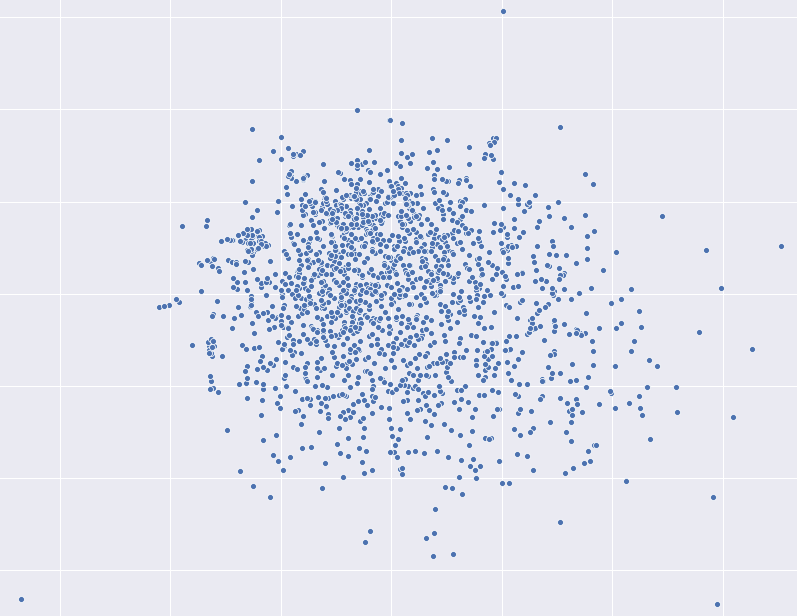
\includegraphics[width=0.48\textwidth]{img/nonmetric_mds_video_codec}
    }
    \subfigure[Metric \gls{mds}]
    {
        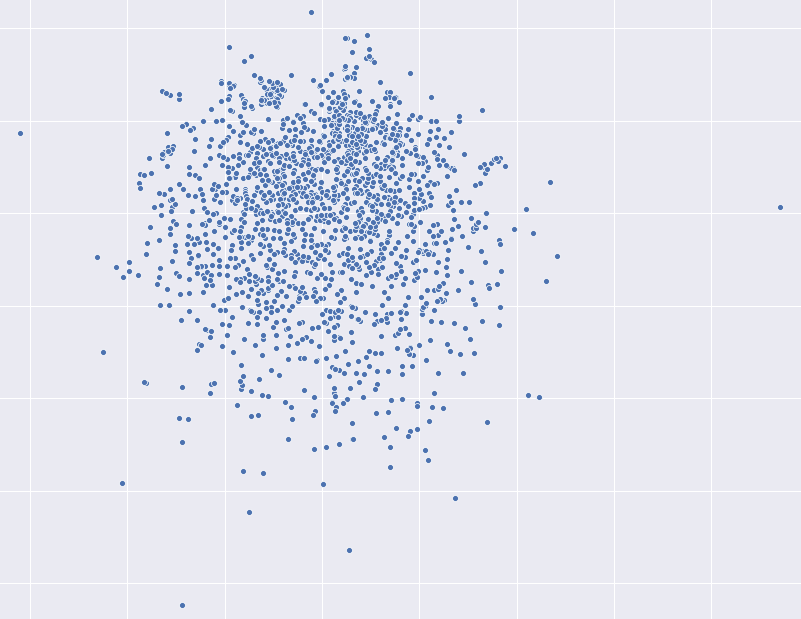
\includegraphics[width=0.48\textwidth]{img/metric_mds_video_codec}
    }\\
    \subfigure[Isomap. Straight lines represent patent families.]
    {
        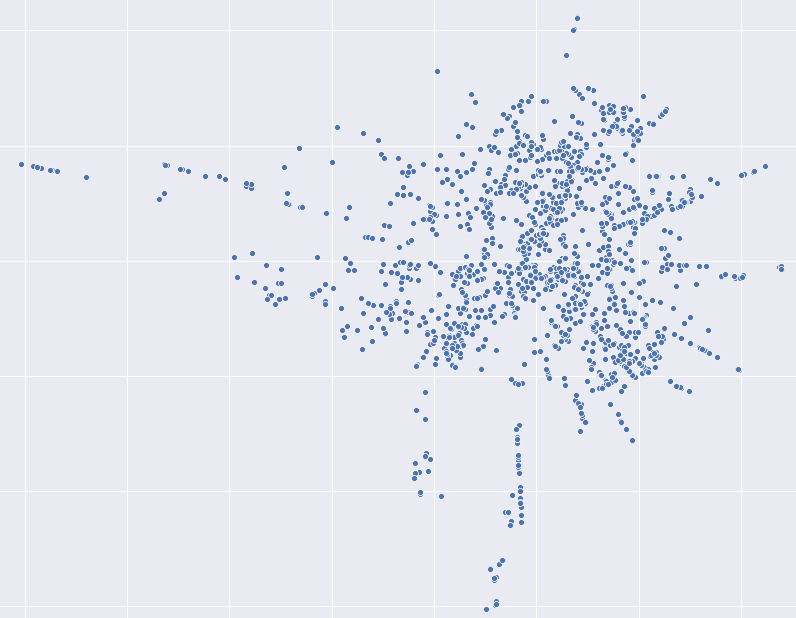
\includegraphics[width=0.48\textwidth]{img/isomap_video_codec}
    }
    \subfigure[\gls{pca}]
    {
        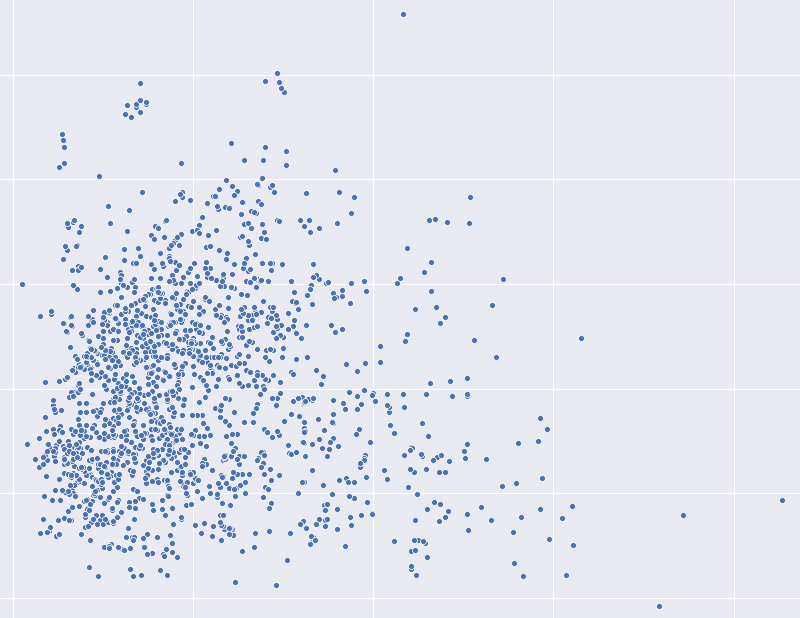
\includegraphics[width=0.48\textwidth]{img/pca_video_codec}
    }
    \caption{A comparison of dimension reduction techniques applied to the video codec dataset.}
    \label{fig:other_dimension_reduction}
\end{figure}

%\section{A comparison of document vectors computed with and without \gls{idf} weighting. Contact lens dataset.}
\begin{figure}[h!]
    \centering
    \subfigure[Non-weighted average]
    {
        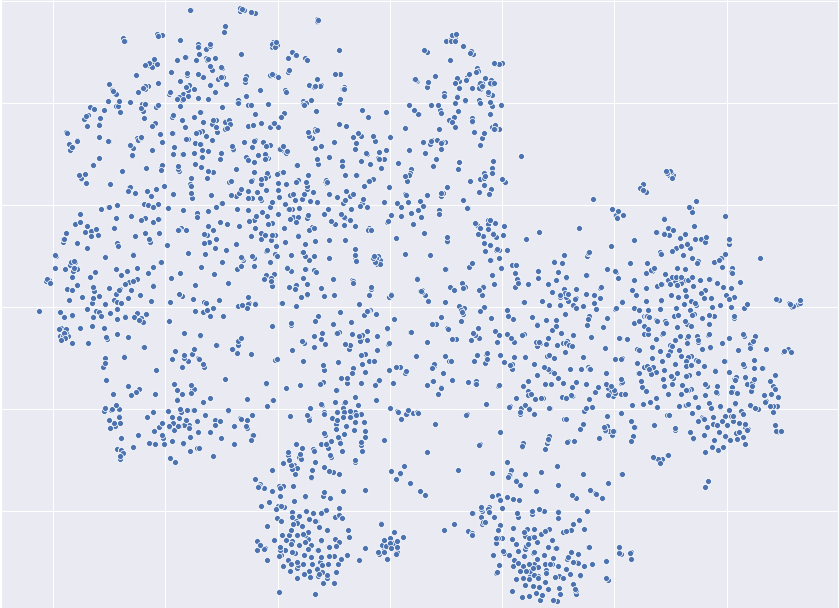
\includegraphics[width=0.95\textwidth]{img/tsne_contact_lens_averaged}
    }\\
    \subfigure[Weighted average]
    {
        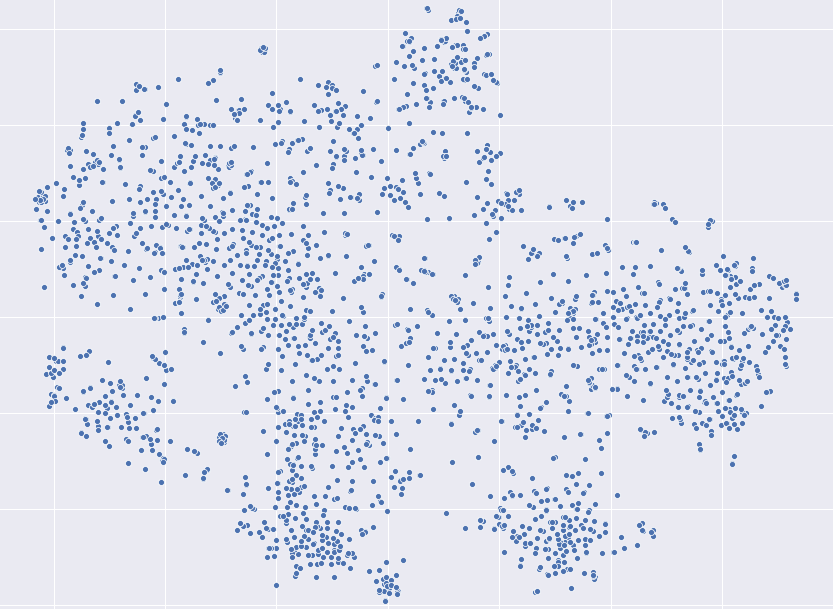
\includegraphics[width=0.95\textwidth]{img/tsne_contact_lens_weighted}
    }
    \caption{A comparison of document vectors computed with and without \gls{idf} weighting. Contact lens dataset.}
    \label{fig:weighted_vs_average_contact_lens}
\end{figure}

%\section{Distribution of text lengths in patent datasets after stopword removal}
\begin{figure}[h!]
    \centering
    \subfigure[Contact lens dataset]
    {
        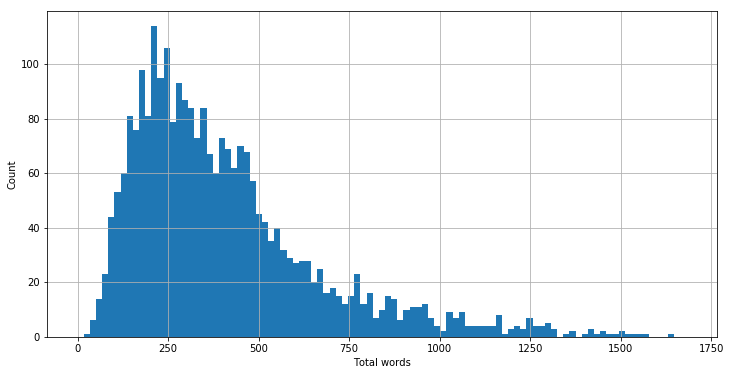
\includegraphics[width=\textwidth]{img/words_contact_lens_us}
        \label{fig:words_contact_lens_us}
    }\\
    \subfigure[Diesel dataset]
    {
	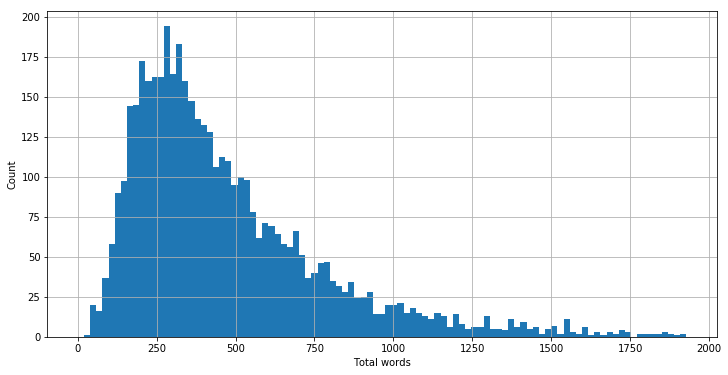
\includegraphics[width=\textwidth]{img/words_diesel}
        \label{fig:words_diesel}
    }
    \caption{Distributions of text length after stopword removal}
    \label{fig:text_length_distributions}
\end{figure}
